\documentclass[aspectratio=169,10pt]{beamer}

\usepackage{fontspec}
\usepackage{booktabs}
\usepackage{amsmath}
\usepackage{siunitx}
\usepackage{tikz}
\usepackage{pgfplots}
\usepackage{ragged2e}
\usepackage{array}
\usepackage{hyperref}

\usetikzlibrary{arrows.meta,calc,positioning,shapes.geometric}
\pgfplotsset{compat=1.18}
\setsansfont{Avenir Next}
\setmonofont{Menlo}
\sisetup{detect-all}

\definecolor{Ink}{HTML}{17212B}
\definecolor{Muted}{HTML}{64717D}
\definecolor{Rule}{HTML}{D8DEE4}
\definecolor{Paper}{HTML}{F7F9FA}
\definecolor{Teal}{HTML}{087F8C}
\definecolor{Coral}{HTML}{D95D4F}
\definecolor{Gold}{HTML}{D69E2E}
\definecolor{Blue}{HTML}{3567A8}
\definecolor{Green}{HTML}{4C956C}
\definecolor{Plum}{HTML}{7B5EA7}
\definecolor{Coal}{HTML}{3E474F}
\definecolor{Oil}{HTML}{C26A4A}
\definecolor{Gas}{HTML}{3F83C5}
\definecolor{Cement}{HTML}{A89B8C}

\setbeamercolor{normal text}{fg=Ink,bg=Paper}
\setbeamercolor{frametitle}{fg=Ink,bg=Paper}
\setbeamercolor{structure}{fg=Teal}
\setbeamercolor{alerted text}{fg=Coral}
\setbeamerfont{frametitle}{size=\Large,series=\bfseries}
\setbeamerfont{title}{size=\fontsize{27}{30}\selectfont,series=\bfseries}
\setbeamerfont{subtitle}{size=\large}
\setbeamerfont{footline}{size=\fontsize{5.5}{6.5}\selectfont}
\setbeamertemplate{navigation symbols}{}
\setbeamertemplate{itemize item}{\color{Teal}\raise0.15ex\hbox{\scriptsize$\blacksquare$}}
\setbeamertemplate{itemize subitem}{\color{Gold}\raise0.1ex\hbox{\tiny$\blacktriangleright$}}
\setbeamertemplate{frametitle}{
  \vspace{0.30cm}
  \insertframetitle\par
  \vspace{0.05cm}
  {\color{Rule}\rule{\textwidth}{0.5pt}}
}
\setbeamertemplate{footline}{
  \leavevmode
  \hbox{%
    \begin{beamercolorbox}[wd=.82\paperwidth,ht=2.8ex,dp=1.1ex,leftskip=.55cm]{normal text}
      \color{Muted}\insertshorttitle
    \end{beamercolorbox}%
    \begin{beamercolorbox}[wd=.18\paperwidth,ht=2.8ex,dp=1.1ex,rightskip=.55cm plus1fil]{normal text}
      \color{Muted}\hfill\insertframenumber\,/\,\inserttotalframenumber
    \end{beamercolorbox}%
  }
}

\newcommand{\source}[1]{%
  \vfill
  {\fontsize{5.2}{6.2}\selectfont\color{Muted}\textbf{Source:} #1\par}
}
\newcommand{\tagbox}[2]{%
  \tikz[baseline=(n.base)]\node[
    fill=#1!10,draw=#1!30,text=#1,rounded corners=1.5pt,
    inner xsep=5pt,inner ysep=2pt,font=\scriptsize\bfseries
  ] (n) {#2};%
}
\newcommand{\metric}[3]{%
  \begin{tikzpicture}
    \node[draw=#3!28,fill=white,rounded corners=2pt,
      minimum width=3.35cm,minimum height=1.12cm,align=left,
      inner xsep=8pt] {
      {\color{#3}\fontsize{17}{18}\selectfont\bfseries #1}\\[-1pt]
      {\color{Muted}\scriptsize #2}
    };
  \end{tikzpicture}
}
\newcommand{\smallhead}[1]{{\color{Muted}\scriptsize\bfseries\MakeUppercase{#1}}}
\newcommand{\keypoint}[2]{%
  \begin{tikzpicture}
    \node[fill=#1!9,draw=#1!25,rounded corners=2pt,
      text width=\linewidth-14pt,align=left,inner sep=7pt] {#2};
  \end{tikzpicture}
}

\title[CO\textsubscript{2} Emissions \& Monitoring]{A Technical Introduction to\\CO\textsubscript{2} Emissions \& Monitoring}
\subtitle{From global inventories to facility-level decisions}
\author{Environmental Data Science Module}
\date{Data coverage: 1990--2023 \quad | \quad Methods reviewed through 2025}

\begin{document}

% 1
\begin{frame}[plain]
  \begin{tikzpicture}[remember picture,overlay]
    \fill[Ink] (current page.south west) rectangle (current page.north east);
    \fill[Teal] (current page.south west) rectangle ([xshift=0.22cm]current page.north west);
    \draw[Teal!55,line width=1.1pt]
      ([xshift=10.8cm,yshift=-1.0cm]current page.north west)
      .. controls +(1.2,-0.5) and +(-1.1,0.4) ..
      ([xshift=15.4cm,yshift=-4.0cm]current page.north west);
    \draw[Gold!65,line width=1.1pt]
      ([xshift=11.3cm,yshift=-1.0cm]current page.north west)
      .. controls +(0.6,-1.2) and +(-1.3,0.4) ..
      ([xshift=14.7cm,yshift=-6.9cm]current page.north west);
    \foreach \x/\y/\c in {11.2/-1.2/Teal,13.1/-2.4/Gold,15.1/-3.9/Coral,12.2/-5.6/Blue,14.6/-6.8/Green}{
      \fill[\c] ([xshift=\x cm,yshift=\y cm]current page.north west) circle (2.7pt);
      \draw[\c!45] ([xshift=\x cm,yshift=\y cm]current page.north west) circle (8pt);
    }
  \end{tikzpicture}
  \vspace{1.12cm}
  {\color{Teal}\smallhead{Technical lecture deck}}\par
  \vspace{0.35cm}
  {\color{white}\usebeamerfont{title}\inserttitle\par}
  \vspace{0.32cm}
  {\color{white!72}\usebeamerfont{subtitle}\insertsubtitle\par}
  \vspace{0.9cm}
  \begin{columns}[T,onlytextwidth]
    \column{0.29\textwidth}
      {\color{white}\Large\bfseries 38.1}\par
      {\color{white!62}\scriptsize Gt CO\textsubscript{2} in 2023\\fossil + industry}
    \column{0.29\textwidth}
      {\color{white}\Large\bfseries 68\%}\par
      {\color{white!62}\scriptsize increase since 1990\\territorial total}
    \column{0.29\textwidth}
      {\color{white}\Large\bfseries 3 layers}\par
      {\color{white!62}\scriptsize inventories, observations,\\inverse modelling}
  \end{columns}
  \vfill
  {\color{white!55}\scriptsize\insertauthor \hfill \insertdate}
\end{frame}

% 2
\begin{frame}[t,shrink=4]{The analytical chain: from signal to action}
  \begin{columns}[T,onlytextwidth]
    \column{0.64\textwidth}
    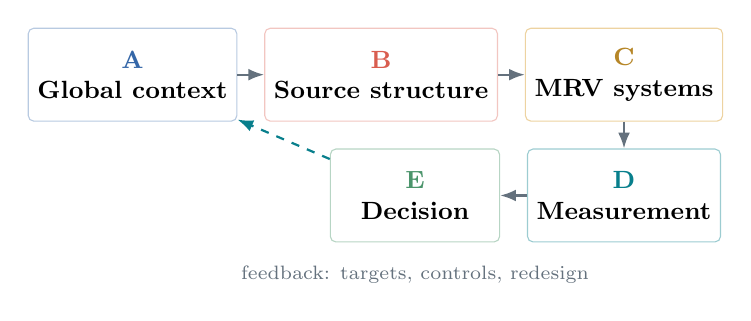
\begin{tikzpicture}[node distance=0.34cm and 0.34cm,
      box/.style={draw=Rule,fill=white,rounded corners=2pt,
        minimum width=2.15cm,minimum height=1.18cm,align=center,font=\small\bfseries},
      arr/.style={-{Latex[length=2mm]},thick,draw=Muted}]
      \node[box,draw=Blue!35] (context) {\color{Blue}A\\Global context};
      \node[box,draw=Coral!35,right=of context] (sources) {\color{Coral}B\\Source structure};
      \node[box,draw=Gold!45,right=of sources] (mrv) {\color{Gold!85!black}C\\MRV systems};
      \node[box,draw=Teal!40,below=of mrv] (methods) {\color{Teal}D\\Measurement};
      \node[box,draw=Green!40,left=of methods] (decision) {\color{Green}E\\Decision};
      \draw[arr] (context) -- (sources);
      \draw[arr] (sources) -- (mrv);
      \draw[arr] (mrv) -- (methods);
      \draw[arr] (methods) -- (decision);
      \draw[arr,dashed,draw=Teal] (decision) -- (context);
      \node[font=\scriptsize,text=Muted,below=0.18cm of decision] {feedback: targets, controls, redesign};
    \end{tikzpicture}
    \vspace{0.28cm}

    \keypoint{Teal}{\textbf{Core question:} What evidence is sufficiently accurate, timely and attributable for the decision being made?}

    \column{0.32\textwidth}
      \smallhead{Three evidence layers}\par\vspace{0.15cm}
      \tagbox{Blue}{1. Estimate}\quad activity $\times$ factor\par\vspace{0.19cm}
      \tagbox{Gold}{2. Observe}\quad concentration / proxy\par\vspace{0.19cm}
      \tagbox{Teal}{3. Reconcile}\quad model + uncertainty\par\vspace{0.43cm}
      {\small
      \textbf{Learning outcomes}\par
      \begin{itemize}\setlength\itemsep{2pt}
        \item Interpret emissions datasets
        \item Design an auditable MRV chain
        \item Match methods to decisions
      \end{itemize}}
  \end{columns}
  \source{\href{https://www.ipcc.ch/working-group/tfi/}{IPCC TFI}; \href{https://ghgprotocol.org/corporate-standard}{GHG Protocol Corporate Standard}.}
\end{frame}

% 3
\begin{frame}[t]{A. Global fossil CO\textsubscript{2}: growth interrupted, not reversed}
  \begin{columns}[T,onlytextwidth]
    \column{0.68\textwidth}
    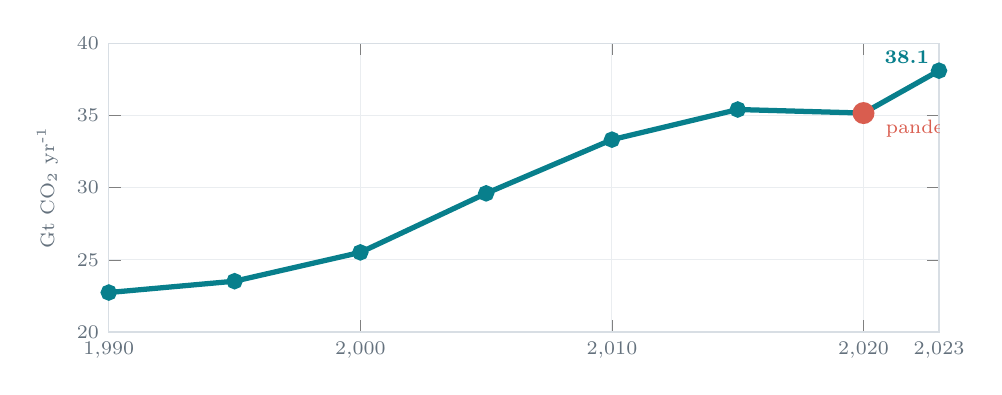
\begin{tikzpicture}
      \begin{axis}[
        width=\linewidth,height=5.25cm,
        xmin=1990,xmax=2023,ymin=20,ymax=40,
        xtick={1990,2000,2010,2020,2023},
        ytick={20,25,30,35,40},
        ylabel={Gt CO\textsubscript{2} yr\textsuperscript{-1}},
        tick label style={font=\scriptsize,color=Muted},
        label style={font=\scriptsize,color=Muted},
        grid=major,grid style={Rule!55},axis line style={Rule},
        every axis plot/.append style={line width=1.9pt}
      ]
        \addplot[Teal,mark=*,mark size=2pt] coordinates {
          (1990,22.732) (1995,23.517) (2000,25.511) (2005,29.599)
          (2010,33.318) (2015,35.404) (2020,35.158) (2023,38.094)
        };
        \addplot[Coral,only marks,mark=*,mark size=3pt] coordinates {(2020,35.158)};
        \node[anchor=west,font=\scriptsize,text=Coral] at (axis cs:2020.5,34.1) {pandemic dip};
        \node[anchor=east,font=\scriptsize\bfseries,text=Teal] at (axis cs:2023,39.0) {38.1};
      \end{axis}
    \end{tikzpicture}
    \column{0.28\textwidth}
      \metric{+68\%}{1990--2023}{Coral}\par\vspace{0.25cm}
      \metric{+5.36}{Gt since 2010}{Gold}\par\vspace{0.25cm}
      \keypoint{Blue}{A temporary shock changed the \textit{level}; it did not establish a sustained downward \textit{trend}.}
  \end{columns}
  \source{Global Carbon Budget (2025), processed by \href{https://ourworldindata.org/grapher/annual-co2-emissions-per-country}{Our World in Data}. Territorial fossil and industrial CO\textsubscript{2}; excludes land-use change.}
\end{frame}

% 4
\begin{frame}[t,shrink=6]{A. Three national pathways, one global accounting problem}
  \begin{columns}[T,onlytextwidth]
    \column{0.67\textwidth}
    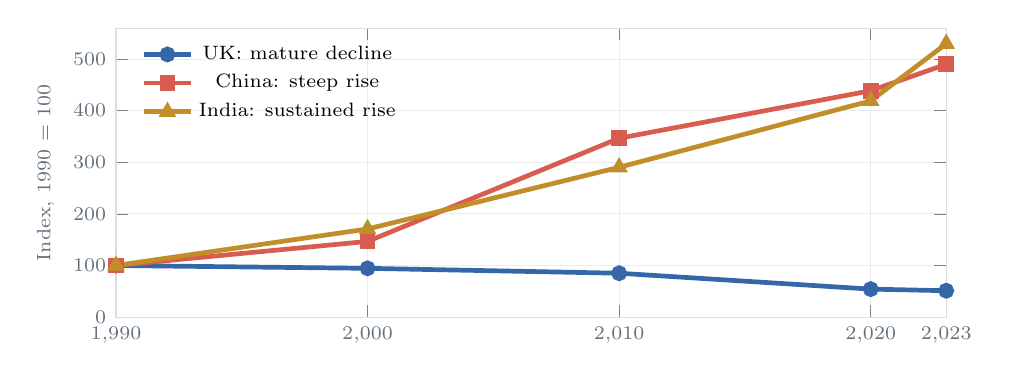
\begin{tikzpicture}
      \begin{axis}[
        width=\linewidth,height=5.25cm,
        xmin=1990,xmax=2023,ymin=0,ymax=560,
        xtick={1990,2000,2010,2020,2023},
        ytick={0,100,200,300,400,500},
        ylabel={Index, 1990 = 100},
        tick label style={font=\scriptsize,color=Muted},
        label style={font=\scriptsize,color=Muted},
        grid=major,grid style={Rule!55},axis line style={Rule},
        legend style={draw=none,fill=none,font=\scriptsize,at={(0.02,0.98)},anchor=north west}
      ]
        \addplot[Blue,line width=1.7pt,mark=*] coordinates {(1990,100)(2000,94.5)(2010,85.0)(2020,54.2)(2023,51.1)};
        \addlegendentry{UK: mature decline}
        \addplot[Coral,line width=1.7pt,mark=square*] coordinates {(1990,100)(2000,146.7)(2010,346.7)(2020,438.8)(2023,490.1)};
        \addlegendentry{China: steep rise}
        \addplot[Gold!90!black,line width=1.7pt,mark=triangle*] coordinates {(1990,100)(2000,170.8)(2010,290.4)(2020,419.2)(2023,529.9)};
        \addlegendentry{India: sustained rise}
      \end{axis}
    \end{tikzpicture}
    \column{0.29\textwidth}
      \smallhead{Do not infer causality from shape alone}\par\vspace{0.18cm}
      {\small
      \begin{itemize}\setlength\itemsep{5pt}
        \item Industrial structure
        \item Energy access and demand
        \item Trade displacement
        \item Policy and technology
      \end{itemize}}
      \vspace{0.22cm}
      \keypoint{Teal}{Normalize for trajectory; retain absolute tonnes for climate relevance.}
  \end{columns}
  \source{Global Carbon Budget (2025) via \href{https://ourworldindata.org/grapher/annual-co2-emissions-per-country}{OWID}. Values are territorial fossil and industrial CO\textsubscript{2}.}
\end{frame}

% 5
\begin{frame}[t]{A. The metric defines the claim}
  \begin{columns}[T,onlytextwidth]
    \column{0.58\textwidth}
    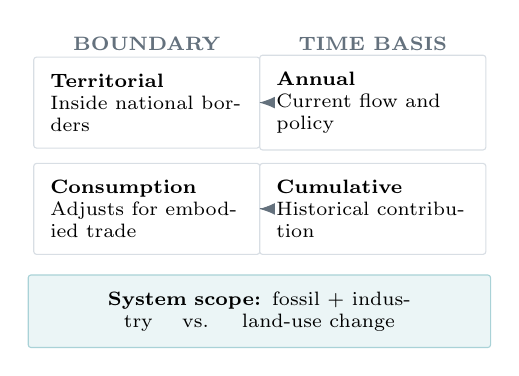
\begin{tikzpicture}[
      cell/.style={draw=Rule,fill=white,rounded corners=1pt,
        text width=2.45cm,minimum height=1.12cm,align=left,inner sep=6pt,font=\scriptsize},
      head/.style={font=\scriptsize\bfseries,text=Muted}]
      \node[head] at (1.25,3.75) {BOUNDARY};
      \node[head] at (4.12,3.75) {TIME BASIS};
      \node[cell] (terr) at (1.25,3.0) {\textbf{Territorial}\\Inside national borders};
      \node[cell] (cons) at (1.25,1.65) {\textbf{Consumption}\\Adjusts for embodied trade};
      \node[cell] (annual) at (4.12,3.0) {\textbf{Annual}\\Current flow and policy};
      \node[cell] (cumul) at (4.12,1.65) {\textbf{Cumulative}\\Historical contribution};
      \node[draw=Teal!35,fill=Teal!8,rounded corners=1pt,
        text width=5.45cm,align=center,inner sep=6pt,font=\scriptsize] at (2.68,0.35)
        {\textbf{System scope:} fossil + industry \quad vs. \quad land-use change};
      \draw[-{Latex[length=2mm]},Muted] (terr) -- (annual);
      \draw[-{Latex[length=2mm]},Muted] (cons) -- (cumul);
    \end{tikzpicture}
    \column{0.38\textwidth}
      \smallhead{A defensible chart states}\par\vspace{0.15cm}
      {\small
      \begin{enumerate}\setlength\itemsep{5pt}
        \item Gas and warming metric
        \item Organizational/geographic boundary
        \item Time period and revision
        \item Included/excluded sources
      \end{enumerate}}
      \vspace{0.18cm}
      \keypoint{Coral}{“CO\textsubscript{2} emissions” is not a complete variable definition.}
  \end{columns}
  \source{\href{https://ourworldindata.org/co2-dataset-sources}{OWID data sources and methods}; \href{https://globalcarbonbudget.org/gcb-2024/faqs/}{Global Carbon Budget FAQ}.}
\end{frame}

% 6
\begin{frame}[t]{B. Major emitters: scale is concentrated, responsibility is multidimensional}
  \begin{columns}[T,onlytextwidth]
    \column{0.68\textwidth}
    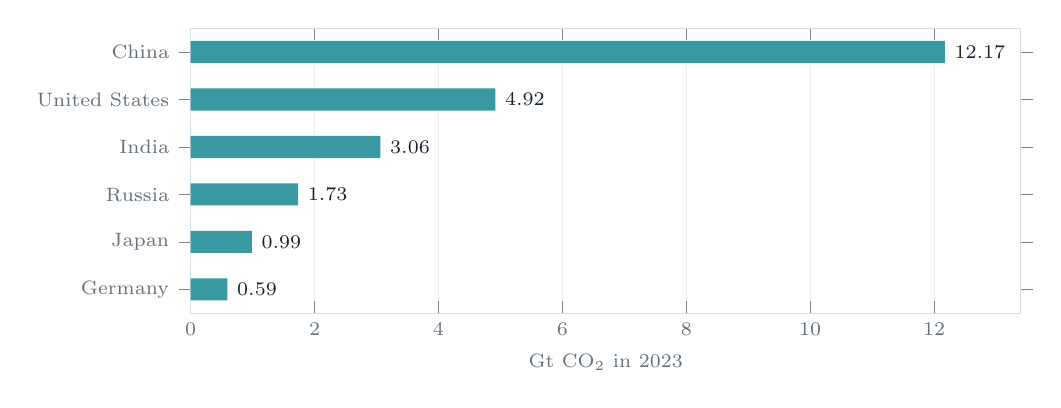
\begin{tikzpicture}
      \begin{axis}[
        xbar,width=\linewidth,height=5.2cm,
        xmin=0,xmax=13.4,
        symbolic y coords={Germany,Japan,Russia,India,United States,China},
        ytick=data,
        xlabel={Gt CO\textsubscript{2} in 2023},
        tick label style={font=\scriptsize,color=Muted},
        label style={font=\scriptsize,color=Muted},
        xmajorgrids=true,grid style={Rule!55},
        axis line style={Rule},
        nodes near coords,
        nodes near coords style={font=\scriptsize\bfseries,color=Ink},
        bar width=8pt
      ]
        \addplot[fill=Teal!80,draw=none] coordinates {
          (0.594,Germany)(0.987,Japan)(1.733,Russia)
          (3.063,India)(4.918,United States)(12.172,China)
        };
      \end{axis}
    \end{tikzpicture}
    \column{0.28\textwidth}
      \metric{60.8\%}{top three share}{Teal}\par\vspace{0.25cm}
      \smallhead{Complementary lenses}\par\vspace{0.14cm}
      \tagbox{Blue}{Per capita}\par\vspace{0.15cm}
      \tagbox{Gold}{Cumulative}\par\vspace{0.15cm}
      \tagbox{Coral}{Consumption-based}\par\vspace{0.3cm}
      {\scriptsize\color{Muted}The ranking changes with the policy question; the atmosphere responds to the total.}
  \end{columns}
  \source{Global Carbon Budget (2025) via \href{https://ourworldindata.org/grapher/annual-co2-emissions-per-country}{OWID}; world total = 38.094 Gt CO\textsubscript{2}.}
\end{frame}

% 7
\begin{frame}[t]{B. Sector structure: direct emissions and electricity attribution}
  \begin{columns}[T,onlytextwidth]
    \column{0.55\textwidth}
    \smallhead{Direct global GHG emissions, 2019}\par\vspace{0.18cm}
    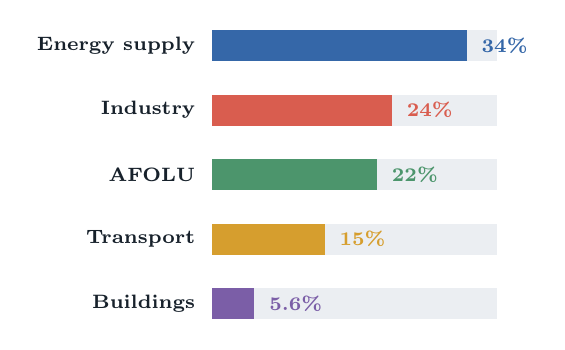
\begin{tikzpicture}[x=0.095cm,y=0.82cm]
      \foreach \name/\value/\y/\col in {
        {Energy supply}/34/4/Blue,
        {Industry}/24/3/Coral,
        {AFOLU}/22/2/Green,
        {Transport}/15/1/Gold,
        {Buildings}/5.6/0/Plum}{
        \fill[Rule!50] (0,\y) rectangle (38,\y+0.48);
        \fill[\col] (0,\y) rectangle (\value,\y+0.48);
        \node[anchor=east,font=\scriptsize\bfseries,text=Ink] at (-1,\y+0.24) {\name};
        \node[anchor=west,font=\scriptsize\bfseries,text=\col] at (\value+0.7,\y+0.24) {\value\%};
      }
    \end{tikzpicture}
    \column{0.41\textwidth}
      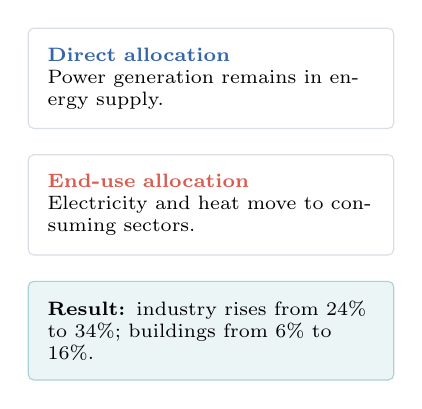
\begin{tikzpicture}[node distance=0.32cm,
        box/.style={draw=Rule,fill=white,rounded corners=2pt,text width=4.15cm,inner sep=7pt,font=\scriptsize}]
        \node[box] (direct) {\textbf{\color{Blue}Direct allocation}\\Power generation remains in energy supply.};
        \node[box,below=of direct] (realloc) {\textbf{\color{Coral}End-use allocation}\\Electricity and heat move to consuming sectors.};
        \node[draw=Teal!35,fill=Teal!8,rounded corners=2pt,
          below=of realloc,text width=4.15cm,inner sep=7pt,font=\scriptsize]
          {\textbf{Result:} industry rises from 24\% to 34\%; buildings from 6\% to 16\%.};
      \end{tikzpicture}
  \end{columns}
  \source{\href{https://www.ipcc.ch/report/ar6/wg3/chapter/chapter-2/}{IPCC AR6 WGIII, Ch. 2}; sector shares are GHG in CO\textsubscript{2}e, not CO\textsubscript{2} alone.}
\end{frame}

% 8
\begin{frame}[t]{B. Fuel decomposition: coal remains the largest component}
  \begin{columns}[T,onlytextwidth]
    \column{0.69\textwidth}
    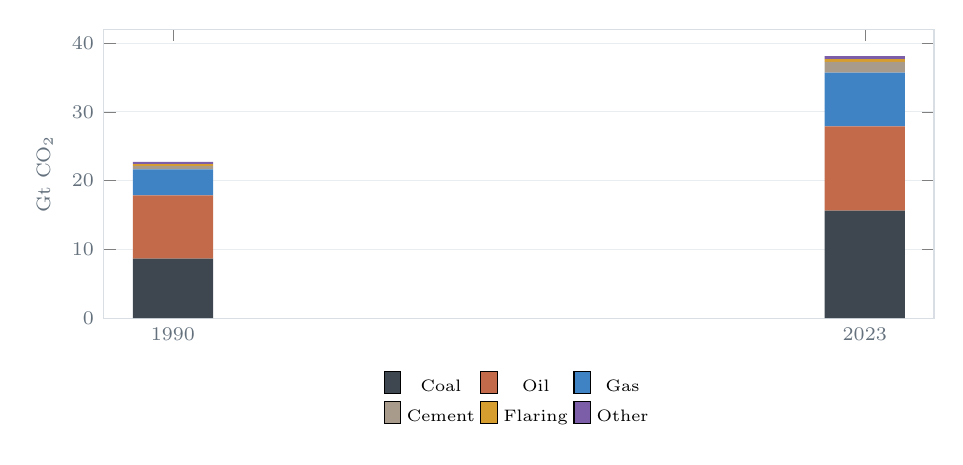
\begin{tikzpicture}
      \begin{axis}[
        ybar stacked,width=\linewidth,height=5.25cm,
        ymin=0,ymax=42,
        symbolic x coords={1990,2023},xtick=data,
        ylabel={Gt CO\textsubscript{2}},
        tick label style={font=\scriptsize,color=Muted},
        label style={font=\scriptsize,color=Muted},
        axis line style={Rule},ymajorgrids=true,grid style={Rule!55},
        bar width=29pt,
        legend style={draw=none,fill=none,font=\fontsize{6.2}{7}\selectfont,
          at={(0.5,-0.16)},anchor=north,legend columns=3}
      ]
        \addplot[fill=Coal,draw=none] coordinates {(1990,8.660)(2023,15.636)};
        \addlegendentry{Coal}
        \addplot[fill=Oil,draw=none] coordinates {(1990,9.196)(2023,12.278)};
        \addlegendentry{Oil}
        \addplot[fill=Gas,draw=none] coordinates {(1990,3.790)(2023,7.803)};
        \addlegendentry{Gas}
        \addplot[fill=Cement,draw=none] coordinates {(1990,0.493)(2023,1.540)};
        \addlegendentry{Cement}
        \addplot[fill=Gold,draw=none] coordinates {(1990,0.257)(2023,0.411)};
        \addlegendentry{Flaring}
        \addplot[fill=Plum,draw=none] coordinates {(1990,0.336)(2023,0.425)};
        \addlegendentry{Other}
      \end{axis}
    \end{tikzpicture}
    \column{0.27\textwidth}
      \metric{41.1\%}{coal share, 2023}{Coal}\par\vspace{0.22cm}
      \metric{32.2\%}{oil share, 2023}{Oil}\par\vspace{0.22cm}
      \metric{20.5\%}{gas share, 2023}{Gas}\par\vspace{0.2cm}
      {\scriptsize\color{Muted}Fuel totals expose the physical levers behind the aggregate trend.}
  \end{columns}
  \source{Global Carbon Budget (2025) via \href{https://ourworldindata.org/grapher/co2-emissions-by-fuel-line}{OWID fuel series}. Values may not sum exactly due to rounding.}
\end{frame}

% 9
\begin{frame}[t]{C. MRV is an evidence architecture, not a single dataset}
  \begin{columns}[T,onlytextwidth]
    \column{0.58\textwidth}
    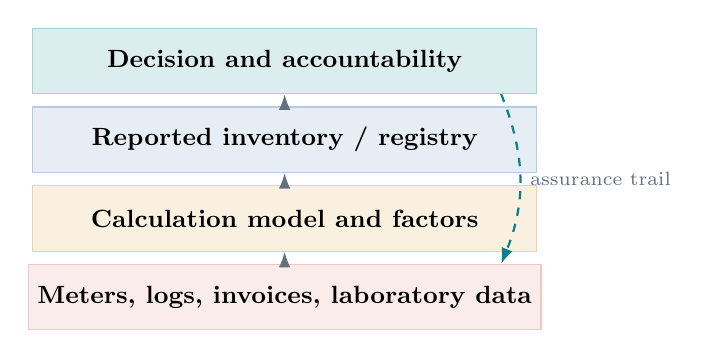
\begin{tikzpicture}[
      level/.style={minimum width=6.4cm,minimum height=0.83cm,align=center,font=\small\bfseries},
      arr/.style={-{Latex[length=2mm]},thick,draw=Muted}]
      \node[level,fill=Teal!14,draw=Teal!35] (dec) at (0,3.45) {Decision and accountability};
      \node[level,fill=Blue!12,draw=Blue!35] (rep) at (0,2.45) {Reported inventory / registry};
      \node[level,fill=Gold!15,draw=Gold!45] (calc) at (0,1.45) {Calculation model and factors};
      \node[level,fill=Coral!12,draw=Coral!35] (raw) at (0,0.45) {Meters, logs, invoices, laboratory data};
      \draw[arr] (raw) -- (calc);
      \draw[arr] (calc) -- (rep);
      \draw[arr] (rep) -- (dec);
      \draw[arr,dashed,draw=Teal] ([xshift=2.75cm]dec.south) to[bend left=22]
        node[right,font=\scriptsize,text=Muted]{assurance trail} ([xshift=2.75cm]raw.north);
    \end{tikzpicture}
    \column{0.38\textwidth}
      \smallhead{Minimum audit fields}\par\vspace{0.12cm}
      {\small
      \begin{itemize}\setlength\itemsep{4pt}
        \item Source identity and owner
        \item Method, factor and version
        \item Unit and temporal coverage
        \item Missing-data treatment
        \item Reviewer and evidence link
      \end{itemize}}
      \vspace{0.18cm}
      \keypoint{Coral}{A precise number without provenance is weak evidence.}
  \end{columns}
  \source{\href{https://ghgprotocol.org/corporate-standard}{GHG Protocol}; \href{https://www.iso.org/obp/ui/en/\#iso:std:66453:en}{ISO 14064-1:2018}; \href{https://www.ipcc.ch/working-group/tfi/}{IPCC TFI}.}
\end{frame}

% 10
\begin{frame}[t]{C. Corporate boundaries: GHG Protocol and ISO 14064-1}
  \begin{columns}[T,onlytextwidth]
    \column{0.61\textwidth}
    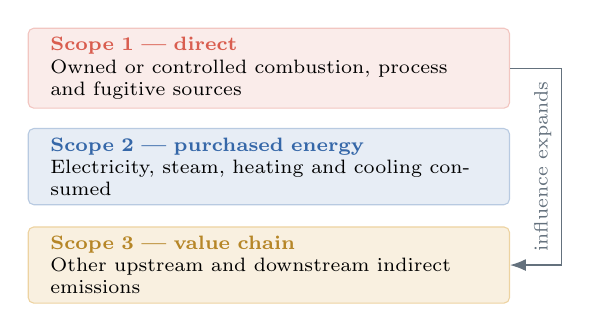
\begin{tikzpicture}[
      scope/.style={rounded corners=2pt,minimum width=5.9cm,minimum height=0.95cm,
        align=left,text width=5.55cm,inner xsep=8pt,font=\scriptsize}]
      \node[scope,fill=Coral!12,draw=Coral!35] (s1) at (0,3.4)
        {\textbf{\color{Coral}Scope 1 | direct}\\Owned or controlled combustion, process and fugitive sources};
      \node[scope,fill=Blue!12,draw=Blue!35] (s2) at (0,2.15)
        {\textbf{\color{Blue}Scope 2 | purchased energy}\\Electricity, steam, heating and cooling consumed};
      \node[scope,fill=Gold!15,draw=Gold!45] (s3) at (0,0.9)
        {\textbf{\color{Gold!85!black}Scope 3 | value chain}\\Other upstream and downstream indirect emissions};
      \draw[-{Latex[length=2mm]},Muted] (s1.east) -- ++(0.65,0) |- (s3.east);
      \node[font=\scriptsize,text=Muted,rotate=90] at (3.48,2.15) {influence expands};
    \end{tikzpicture}
    \column{0.35\textwidth}
      \smallhead{ISO inventory principles}\par\vspace{0.12cm}
      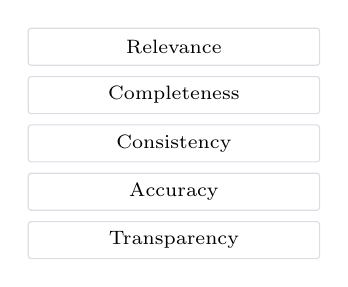
\begin{tikzpicture}[node distance=0.13cm,
        p/.style={draw=Rule,fill=white,rounded corners=1pt,
          minimum width=3.7cm,minimum height=0.47cm,font=\scriptsize,align=center}]
        \node[p] (r) {Relevance};
        \node[p,below=of r] (c) {Completeness};
        \node[p,below=of c] (co) {Consistency};
        \node[p,below=of co] (a) {Accuracy};
        \node[p,below=of a] (t) {Transparency};
      \end{tikzpicture}
      \vspace{0.23cm}
      \keypoint{Teal}{Boundary choice precedes calculation; verification tests the declared boundary.}
  \end{columns}
  \source{\href{https://www.ghgprotocol.org/corporate-standard-frequently-asked-questions}{GHG Protocol scope definitions}; \href{https://www.iso.org/obp/ui/en/\#iso:std:66453:en}{ISO 14064-1:2018}.}
\end{frame}

% 11
\begin{frame}[t]{C. Verified registries convert calculations into compliance evidence}
  \begin{columns}[T,onlytextwidth]
    \column{0.54\textwidth}
      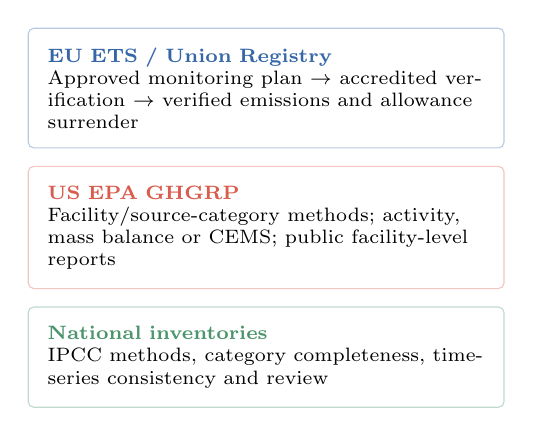
\begin{tikzpicture}[node distance=0.22cm,
        card/.style={draw=Rule,fill=white,rounded corners=2pt,text width=5.55cm,
          minimum height=1.18cm,align=left,inner sep=7pt,font=\scriptsize}]
        \node[card,draw=Blue!35] (eu) {
          \textbf{\color{Blue}EU ETS / Union Registry}\\
          Approved monitoring plan $\rightarrow$ accredited verification $\rightarrow$
          verified emissions and allowance surrender
        };
        \node[card,draw=Coral!35,below=of eu] (us) {
          \textbf{\color{Coral}US EPA GHGRP}\\
          Facility/source-category methods; activity, mass balance or CEMS;
          public facility-level reports
        };
        \node[card,draw=Green!35,below=of us] (nat) {
          \textbf{\color{Green}National inventories}\\
          IPCC methods, category completeness, time-series consistency and review
        };
      \end{tikzpicture}
    \column{0.42\textwidth}
      \smallhead{Annual compliance cycle}\par\vspace{0.14cm}
      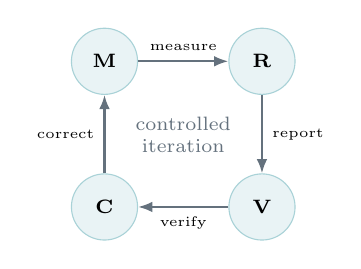
\begin{tikzpicture}[
        cycstep/.style={circle,draw=Teal!35,fill=Teal!9,minimum size=0.84cm,font=\scriptsize\bfseries},
        arr/.style={-{Latex[length=1.8mm]},draw=Muted,thick}]
        \node[cycstep] (m) at (0,2.4) {M};
        \node[cycstep] (r) at (2.0,2.4) {R};
        \node[cycstep] (v) at (2.0,0.55) {V};
        \node[cycstep] (c) at (0,0.55) {C};
        \draw[arr] (m) -- node[above,font=\tiny]{measure} (r);
        \draw[arr] (r) -- node[right,font=\tiny]{report} (v);
        \draw[arr] (v) -- node[below,font=\tiny]{verify} (c);
        \draw[arr] (c) -- node[left,font=\tiny]{correct} (m);
        \node[font=\scriptsize,text=Muted,align=center] at (1,1.47) {controlled\\iteration};
      \end{tikzpicture}
      \vspace{0.15cm}
      \keypoint{Gold}{Verification is risk-based assurance, not proof of zero error.}
  \end{columns}
  \source{\href{https://climate.ec.europa.eu/eu-action/carbon-markets/eu-emissions-trading-system-eu-ets/monitoring-reporting-and-verification_en}{EU ETS MRV}; \href{https://www.epa.gov/ghgreporting}{US EPA GHGRP}; \href{https://www.ipcc.ch/working-group/tfi/}{IPCC TFI}.}
\end{frame}

% 12
\begin{frame}[t]{C. Example: auditable CO\textsubscript{2} workflow for a steel facility}
  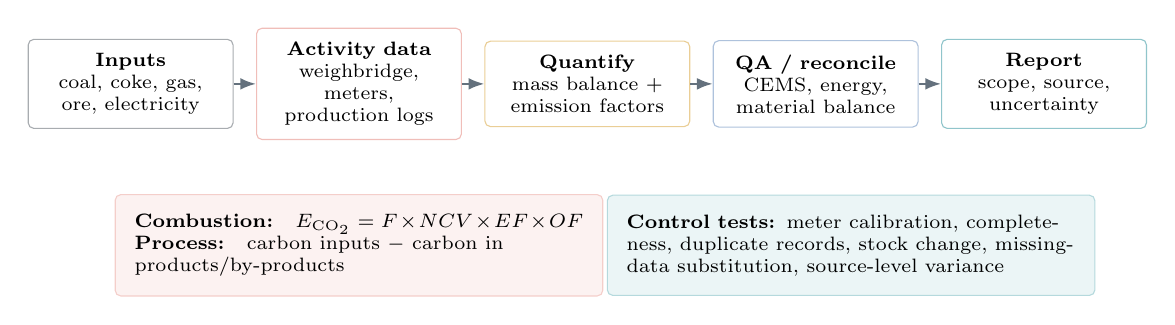
\begin{tikzpicture}[
    box/.style={draw=Rule,fill=white,rounded corners=2pt,text width=2.25cm,
      minimum height=1.05cm,align=center,inner sep=5pt,font=\scriptsize},
    arr/.style={-{Latex[length=2mm]},thick,draw=Muted}]
    \node[box,draw=Coal!45] (inputs) at (0,2.8) {\textbf{Inputs}\\coal, coke, gas,\\ore, electricity};
    \node[box,draw=Coral!40] (activity) at (2.9,2.8) {\textbf{Activity data}\\weighbridge, meters,\\production logs};
    \node[box,draw=Gold!50] (model) at (5.8,2.8) {\textbf{Quantify}\\mass balance +\\emission factors};
    \node[box,draw=Blue!40] (qa) at (8.7,2.8) {\textbf{QA / reconcile}\\CEMS, energy,\\material balance};
    \node[box,draw=Teal!45] (report) at (11.6,2.8) {\textbf{Report}\\scope, source,\\uncertainty};
    \draw[arr] (inputs) -- (activity);
    \draw[arr] (activity) -- (model);
    \draw[arr] (model) -- (qa);
    \draw[arr] (qa) -- (report);
    \node[draw=Coral!30,fill=Coral!8,rounded corners=2pt,text width=5.7cm,
      align=left,inner sep=7pt,font=\scriptsize] at (2.9,0.75) {
      \textbf{Combustion:}\quad $E_{\mathrm{CO_2}} = F \times NCV \times EF \times OF$\\
      \textbf{Process:}\quad carbon inputs $-$ carbon in products/by-products
    };
    \node[draw=Teal!30,fill=Teal!8,rounded corners=2pt,text width=5.7cm,
      align=left,inner sep=7pt,font=\scriptsize] at (9.15,0.75) {
      \textbf{Control tests:} meter calibration, completeness, duplicate records,
      stock change, missing-data substitution, source-level variance
    };
  \end{tikzpicture}
  \source{\href{https://www.epa.gov/ghgreporting/subpart-q-information-sheet}{US EPA GHGRP Subpart Q}; \href{https://climatetrace.org/news/conversations-with-the-coalition-transitionzero}{Climate TRACE heavy-industry methods}; GHG Protocol Corporate Standard.}
\end{frame}

% 13
\begin{frame}[t]{D. Bottom-up techniques: choose the closest measurable driver}
  \begin{columns}[T,onlytextwidth]
    \column{0.59\textwidth}
    \scriptsize
    \renewcommand{\arraystretch}{1.12}
    \begin{tabular}{>{\bfseries}p{1.35cm}p{2.25cm}p{2.55cm}}
      \toprule
      Method & Best use & Dominant limitation\\
      \midrule
      Fuel meter & Combustion sources & Calibration, fuel quality\\
      Mass balance & Carbon-rich processes & Stock and carbon content\\
      CEMS & Large stacks & Representativeness, downtime\\
      Production proxy & Rapid estimates & Technology heterogeneity\\
      Emission factor & Broad inventories & Transferability, vintage\\
      \bottomrule
    \end{tabular}
    \vspace{0.18cm}

    \keypoint{Blue}{Higher-tier methods replace generic factors with source-specific activity, composition or direct measurement.}
    \column{0.37\textwidth}
      \smallhead{Generic model}\par\vspace{0.14cm}
      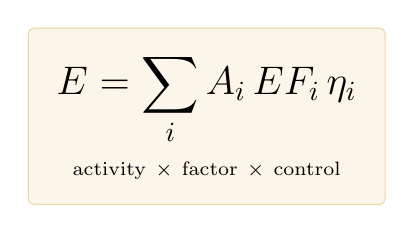
\begin{tikzpicture}
        \node[draw=Gold!40,fill=Gold!10,rounded corners=2pt,
          text width=3.9cm,align=center,inner sep=9pt] {
          \Large $\displaystyle E=\sum_i A_i\,EF_i\,\eta_i$\\[5pt]
          \scriptsize activity $\times$ factor $\times$ control
        };
      \end{tikzpicture}
      \vspace{0.18cm}
      {\scriptsize
      \textbf{Design principle}\par
      Use the simplest method that meets the required materiality, frequency and attribution.}
  \end{columns}
  \source{\href{https://www.ipcc.ch/working-group/tfi/}{IPCC inventory methodologies}; \href{https://www.ipcc-nggip.iges.or.jp/efdb/}{IPCC Emission Factor Database}; \href{https://www.epa.gov/ghgreporting}{US EPA GHGRP}.}
\end{frame}

% 14
\begin{frame}[t]{D. Satellites observe atmospheric columns, not ledger entries}
  \begin{columns}[T,onlytextwidth]
    \column{0.59\textwidth}
    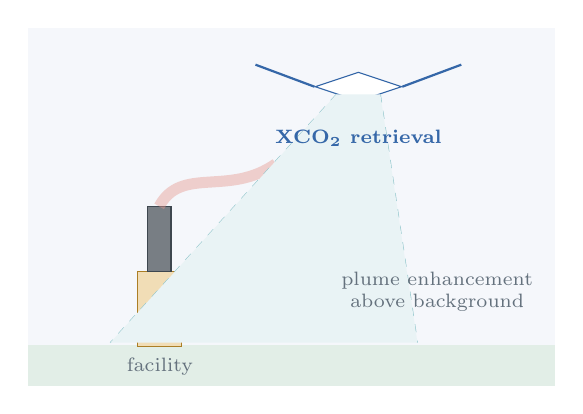
\begin{tikzpicture}
      \fill[Blue!5] (-0.4,0) rectangle (6.3,4.55);
      \fill[Green!16] (-0.4,0) rectangle (6.3,0.52);
      \node[diamond,aspect=1.7,draw=Blue,fill=white,minimum width=1.1cm] (sat) at (3.8,3.8) {};
      \draw[Blue,thick] (sat.west) -- ++(-0.75,0.28);
      \draw[Blue,thick] (sat.east) -- ++(0.75,0.28);
      \draw[Gold!80!black,fill=Gold!35] (1.0,0.5) rectangle (1.55,1.45);
      \draw[Coal,fill=Coal!70] (1.12,1.45) rectangle (1.42,2.28);
      \draw[Coral!65,line width=4pt,opacity=.42] (1.27,2.28)
        .. controls (1.55,2.8) and (2.15,2.4) .. (2.75,2.82);
      \draw[Teal!45,dashed] (sat.south west) -- (0.65,0.55);
      \draw[Teal!45,dashed] (sat.south east) -- (4.55,0.55);
      \fill[Teal!9] (0.65,0.55) -- (4.55,0.55) -- (sat.south east) -- (sat.south west) -- cycle;
      \node[font=\scriptsize\bfseries,text=Blue] at (3.8,3.15) {XCO\textsubscript{2} retrieval};
      \node[font=\scriptsize,text=Muted,align=center] at (4.8,1.2)
        {plume enhancement\\above background};
      \node[font=\scriptsize,text=Muted] at (1.28,0.25) {facility};
    \end{tikzpicture}
    \column{0.37\textwidth}
      \smallhead{What the signal requires}\par\vspace{0.12cm}
      \tagbox{Blue}{Column concentration}\par\vspace{0.14cm}
      \tagbox{Gold}{Wind / transport}\par\vspace{0.14cm}
      \tagbox{Coral}{Background estimate}\par\vspace{0.14cm}
      \tagbox{Teal}{Cloud / aerosol screening}\par\vspace{0.28cm}
      {\scriptsize
      \textbf{OCO-2/OCO-3:} CO\textsubscript{2} column retrievals.\\
      \textbf{Sentinel-5P:} daily trace-gas context (CO, NO\textsubscript{2}, CH\textsubscript{4}, etc.), not a CO\textsubscript{2} product.}
  \end{columns}
  \source{\href{https://ocov2.jpl.nasa.gov/}{NASA OCO-2}; \href{https://dataspace.copernicus.eu/explore-data/data-collections/sentinel-data/sentinel-5p}{Copernicus Sentinel-5P}; Nassar et al. (2022), \href{https://doi.org/10.3389/frsen.2022.1028240}{doi:10.3389/frsen.2022.1028240}.}
\end{frame}

% 15
\begin{frame}[t]{D. Top-down inversion and near-real-time nowcasting answer different questions}
  \begin{columns}[T,onlytextwidth]
    \column{0.62\textwidth}
    \smallhead{Atmospheric inversion}\par\vspace{0.12cm}
    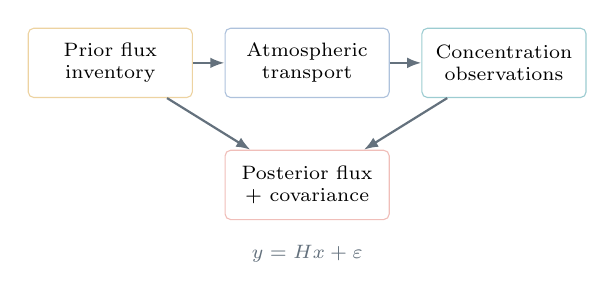
\begin{tikzpicture}[
      box/.style={draw=Rule,fill=white,rounded corners=2pt,text width=1.85cm,
        minimum height=0.88cm,align=center,font=\scriptsize},
      arr/.style={-{Latex[length=1.8mm]},thick,draw=Muted}]
      \node[box,draw=Gold!45] (prior) at (0,2.8) {Prior flux\\inventory};
      \node[box,draw=Blue!40] (transport) at (2.5,2.8) {Atmospheric\\transport};
      \node[box,draw=Teal!40] (obs) at (5.0,2.8) {Concentration\\observations};
      \node[box,draw=Coral!40] (post) at (2.5,1.25) {Posterior flux\\+ covariance};
      \draw[arr] (prior) -- (transport);
      \draw[arr] (transport) -- (obs);
      \draw[arr] (obs) -- (post);
      \draw[arr] (prior) -- (post);
      \node[font=\scriptsize,text=Muted] at (2.5,0.38) {$y = Hx + \varepsilon$};
    \end{tikzpicture}
    \column{0.34\textwidth}
      \smallhead{Carbon Monitor nowcast}\par\vspace{0.12cm}
      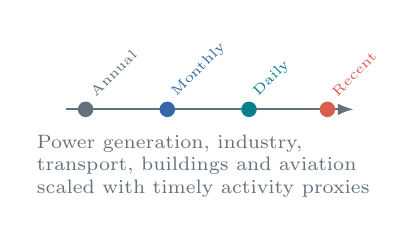
\begin{tikzpicture}[x=0.83cm,y=0.72cm]
        \draw[Muted,thick,-{Latex[length=2mm]}] (0,0) -- (4.4,0);
        \foreach \x/\lab/\col in {0.3/Annual/Muted,1.55/Monthly/Blue,2.8/Daily/Teal,4.0/Recent/Coral}{
          \fill[\col] (\x,0) circle (2.8pt);
          \node[font=\tiny,text=\col,rotate=45,anchor=west] at (\x,0.15) {\lab};
        }
        \node[font=\scriptsize,text=Muted,align=left] at (2.1,-1.0)
          {Power generation, industry,\\transport, buildings and aviation\\scaled with timely activity proxies};
      \end{tikzpicture}
      \vspace{0.22cm}
      \keypoint{Gold}{Nowcasts optimize latency; inversions optimize atmospheric consistency.}
  \end{columns}
  \source{\href{https://gml.noaa.gov/ccgg/carbontracker/}{NOAA CarbonTracker}; Liu et al. (2020), \href{https://doi.org/10.1038/s41597-020-00708-7}{Carbon Monitor}; \href{https://carbonmonitor.org/}{carbonmonitor.org}.}
\end{frame}

% 16
\begin{frame}[t,shrink=2]{D. Uncertainty is structured information}
  \begin{columns}[T,onlytextwidth]
    \column{0.56\textwidth}
      \smallhead{Propagation for a simple product}\par\vspace{0.12cm}
      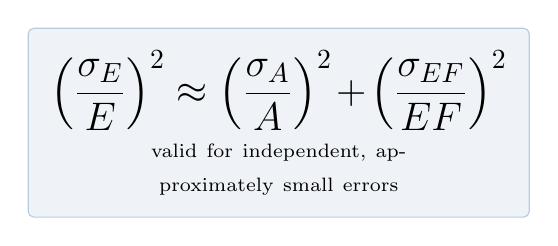
\begin{tikzpicture}
        \node[draw=Blue!35,fill=Blue!8,rounded corners=2pt,
          text width=5.8cm,align=center,inner sep=8pt] {
          \Large $\displaystyle
          \left(\frac{\sigma_E}{E}\right)^2
          \approx
          \left(\frac{\sigma_A}{A}\right)^2+
          \left(\frac{\sigma_{EF}}{EF}\right)^2
          $\\[4pt]
          \scriptsize valid for independent, approximately small errors
        };
      \end{tikzpicture}
      \vspace{0.24cm}
      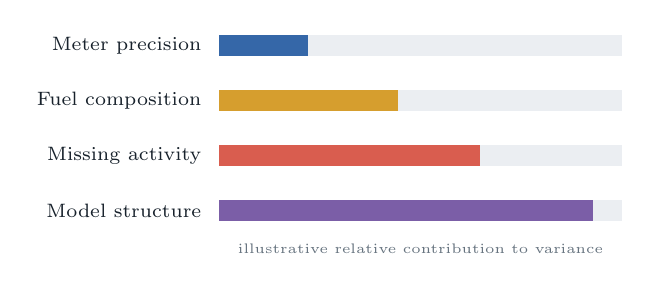
\begin{tikzpicture}[x=0.095cm,y=0.7cm]
        \foreach \name/\value/\y/\col in {
          {Meter precision}/12/3/Blue,
          {Fuel composition}/24/2/Gold,
          {Missing activity}/35/1/Coral,
          {Model structure}/50/0/Plum}{
          \fill[Rule!50] (0,\y) rectangle (54,\y+0.38);
          \fill[\col] (0,\y) rectangle (\value,\y+0.38);
          \node[anchor=east,font=\scriptsize,text=Ink] at (-1,\y+0.19) {\name};
        }
        \node[font=\tiny,text=Muted] at (27,-0.5) {illustrative relative contribution to variance};
      \end{tikzpicture}
    \column{0.40\textwidth}
      \smallhead{Report more than $\pm x\%$}\par\vspace{0.12cm}
      {\small
      \begin{itemize}\setlength\itemsep{4pt}
        \item Random error vs. systematic bias
        \item Correlation across sources and time
        \item Coverage and detection limits
        \item Version and revision uncertainty
        \item Sensitivity to model assumptions
      \end{itemize}}
      \vspace{0.2cm}
      \keypoint{Coral}{Triangulation detects disagreement; it does not automatically identify which estimate is correct.}
  \end{columns}
  \source{\href{https://www.ipcc-nggip.iges.or.jp/faq/faq.html}{IPCC TFI uncertainty FAQ}; Global Carbon Budget 2024 reports fossil CO\textsubscript{2} uncertainty near $\pm5\%$ and substantially larger land-use uncertainty.}
\end{frame}

% 17
\begin{frame}[t]{E. Match the monitoring system to the decision}
  \begin{columns}[T,onlytextwidth]
    \column{0.63\textwidth}
    \scriptsize
    \renewcommand{\arraystretch}{1.12}
    \begin{tabular}{p{1.8cm}p{2.05cm}p{2.55cm}}
      \toprule
      \textbf{Decision} & \textbf{Primary evidence} & \textbf{Critical quality}\\
      \midrule
      National target & Inventory + review & Completeness, consistency\\
      Carbon market & Verified facility MRV & Accuracy, legal traceability\\
      Plant operation & Meter/CEMS nowcast & Latency, source attribution\\
      Supply chain & Supplier primary data & Boundary and allocation\\
      Anomaly detection & Satellite + model & Coverage, false positives\\
      \bottomrule
    \end{tabular}
    \vspace{0.18cm}
    \keypoint{Teal}{The “best” system is the least complex evidence chain that changes the decision reliably.}
    \column{0.33\textwidth}
      \smallhead{Closed-loop action}\par\vspace{0.12cm}
      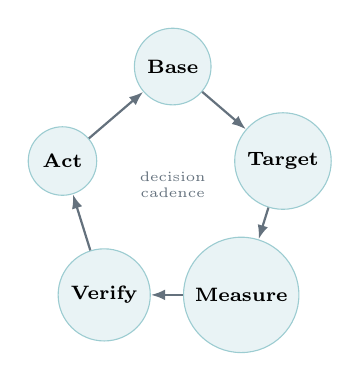
\begin{tikzpicture}[
        n/.style={circle,minimum size=0.87cm,draw=Teal!40,fill=Teal!9,font=\scriptsize\bfseries},
        a/.style={-{Latex[length=1.8mm]},draw=Muted,thick}]
        \node[n] (b) at (1.65,3.25) {Base};
        \node[n] (t) at (3.05,2.05) {Target};
        \node[n] (m) at (2.52,0.35) {Measure};
        \node[n] (v) at (0.78,0.35) {Verify};
        \node[n] (a1) at (0.25,2.05) {Act};
        \draw[a] (b)--(t);
        \draw[a] (t)--(m);
        \draw[a] (m)--(v);
        \draw[a] (v)--(a1);
        \draw[a] (a1)--(b);
        \node[font=\tiny,text=Muted,align=center] at (1.65,1.75) {decision\\cadence};
      \end{tikzpicture}
  \end{columns}
  \source{Synthesis of \href{https://www.ipcc.ch/working-group/tfi/}{IPCC TFI}, \href{https://ghgprotocol.org/corporate-standard}{GHG Protocol}, \href{https://climate.ec.europa.eu/eu-action/carbon-markets/eu-emissions-trading-system-eu-ets/monitoring-reporting-and-verification_en}{EU ETS MRV}, NASA/NOAA and Carbon Monitor methods.}
\end{frame}

% 18
\begin{frame}[t,shrink=7]{E. Takeaway: build a reconciled, decision-grade evidence chain}
  \begin{columns}[T,onlytextwidth]
    \column{0.59\textwidth}
      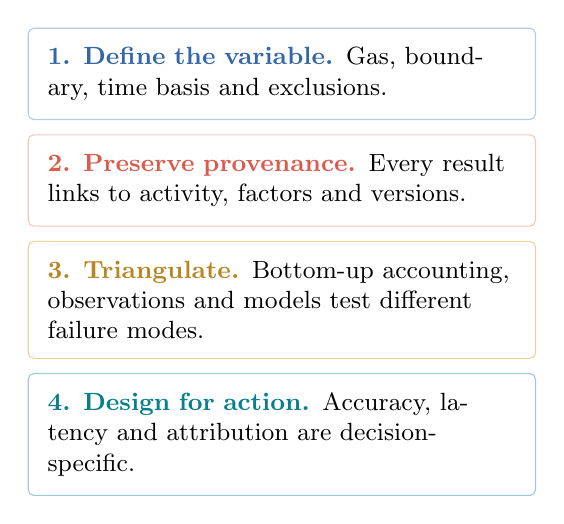
\begin{tikzpicture}[node distance=0.18cm,
        card/.style={draw=Rule,fill=white,rounded corners=2pt,text width=5.95cm,
          minimum height=0.9cm,align=left,inner sep=7pt,font=\small}]
        \node[card,draw=Blue!35] (one) {\textbf{\color{Blue}1. Define the variable.} Gas, boundary, time basis and exclusions.};
        \node[card,draw=Coral!35,below=of one] (two) {\textbf{\color{Coral}2. Preserve provenance.} Every result links to activity, factors and versions.};
        \node[card,draw=Gold!45,below=of two] (three) {\textbf{\color{Gold!85!black}3. Triangulate.} Bottom-up accounting, observations and models test different failure modes.};
        \node[card,draw=Teal!40,below=of three] (four) {\textbf{\color{Teal}4. Design for action.} Accuracy, latency and attribution are decision-specific.};
      \end{tikzpicture}
    \column{0.37\textwidth}
      \smallhead{Reference map}\par\vspace{0.12cm}
      {\scriptsize
      \textbf{Global totals}\\
      \href{https://globalcarbonbudget.org/}{Global Carbon Budget}\\
      \href{https://ourworldindata.org/co2}{Our World in Data}\par\vspace{0.16cm}
      \textbf{Sector and methods}\\
      \href{https://www.ipcc.ch/report/ar6/wg3/}{IPCC AR6 WGIII}\\
      \href{https://edgar.jrc.ec.europa.eu/}{EDGAR / JRC}\par\vspace{0.16cm}
      \textbf{Corporate and compliance}\\
      \href{https://ghgprotocol.org/}{GHG Protocol}\\
      \href{https://www.iso.org/standard/66453.html}{ISO 14064-1}\\
      \href{https://www.epa.gov/ghgreporting}{US EPA GHGRP}\\
      \href{https://climate.ec.europa.eu/eu-action/carbon-markets/eu-emissions-trading-system-eu-ets_en}{EU ETS}\par\vspace{0.16cm}
      \textbf{Observations and rapid estimates}\\
      \href{https://ocov2.jpl.nasa.gov/}{NASA OCO-2}\,;\,
      \href{https://gml.noaa.gov/ccgg/carbontracker/}{NOAA CarbonTracker}\\
      \href{https://carbonmonitor.org/}{Carbon Monitor}\,;\,
      \href{https://climatetrace.org/}{Climate TRACE}}
  \end{columns}
  \vfill
  \begin{center}
    {\color{Ink}\large\bfseries Good monitoring does not merely count carbon.}\\
    {\color{Teal}\large\bfseries It makes claims testable and interventions accountable.}
  \end{center}
\end{frame}

\end{document}
